%==============================================================================
%== template for LATEX poster =================================================
%==============================================================================
%
%--A0 beamer slide-------------------------------------------------------------
\documentclass[final]{beamer}
\usepackage[orientation=portrait,size=a0,
            scale=1.25         % font scale factor
           ]{beamerposter}
\usepackage{graphicx}
\graphicspath{ {images/} }
           
\geometry{
  hmargin=2.5cm, % little modification of margins
}

%
\usepackage[utf8]{inputenc}
\usepackage{physics}

\linespread{1.15}
%
%==The poster style============================================================
\usetheme{sharelatex}

%==Title, date and authors of the poster=======================================
\title
[CANES Retreat 2017] % Conference
{ % Poster title
Understanding Dissipative Control of Quantum Dynamics from Biased Trajectory Ensembles
}

\author{ % Authors
Fergus Barratt\inst{1}
}
\institute
[King's College London] % General University
{
\inst{1} King's College London
}
\date{\today}



\begin{document}
\begin{frame}[t]
%==============================================================================
\begin{multicols}{3}
%==============================================================================
%==The poster content==========================================================
%==============================================================================

\section{Introduction}

\begin[itemize}

\end{itemize}
The technological potential of quantum systems stems from entanglement and the resulting exponential scaling of their state space. Coupling to the environment degrades this entanglement. Understanding how this dissipative degradation of entanglement impacts upon non-equilibrium quantum dynamics is a fundamental problem. The challenge is both one of principle and of a relative dearth of analytical and numerical tools.

This project will apply techniques developed for studying rare fluctuations in non-quantum systems to create novel ways of understanding the effects of dissipation on the dynamics of quantum systems. In particular, we explore the trajectory ensemble approach that was developed in the study of classical glasses. In this approach, the ensemble of trajectories that a system may take is biased – the strength of the bias potentially driving transitions between jammed glassy behaviour and liquid behaviour.

Dissipative effects of the environment have much in common with this trajectory biasing. At its crudest level, a binding brake on a car can bias the trajectory of the car. Similarly, dissipation in quantum systems can favour trajectories in certain directions in Hilbert space. Moreover, these may drive a transition from the presence of desired quantum properties to their absence. We will investigate the application of methods and ideas developed in classical out of equilibrium systems (where Prof. Sollich’s main expertise lies, e.g. in the area of biased trajectory ensembles) to the quantum problem (Prof. Andrew Green’s expertise, including variational approximations and tensor networks).

\section{Trajectory Ensembles}

By analogy to the ensembles of microstates of equilibrium statistical mechanics, in the study of glass forming systems (and elsewhere) ensembles of system trajectories have been studied~\cite{Garrahan2009}.

Starting from Markovian dynamics, the trajectories are biased (as in the canonical ensemble) by the value of some time extensive observable on that trajectory.
At the level of the master equation, this corresponds to a deformation of the operator $\mathbb{W} \rightarrow \mathbb{W}_A$ in the vector form (s is a biasing field, the analogue of $\beta$ the inverse temperature)
\begin{equation}
    \pdv{\vec{P}_A}{t} = \mathbb{W}_A(s) \vec{P}_A,
\end{equation}
and from there for the dynamical analogue of the partition function
\begin{equation}
    \mathcal{Z}_A(s, t) \sim e^{t \psi_A(s)}
\end{equation}
where $\psi_A(s)$ is the largest eigenvalue of the matrix $\mathbb{W}_A(s)$.

\section{Matrix Product States}

\begin{figure}[h]
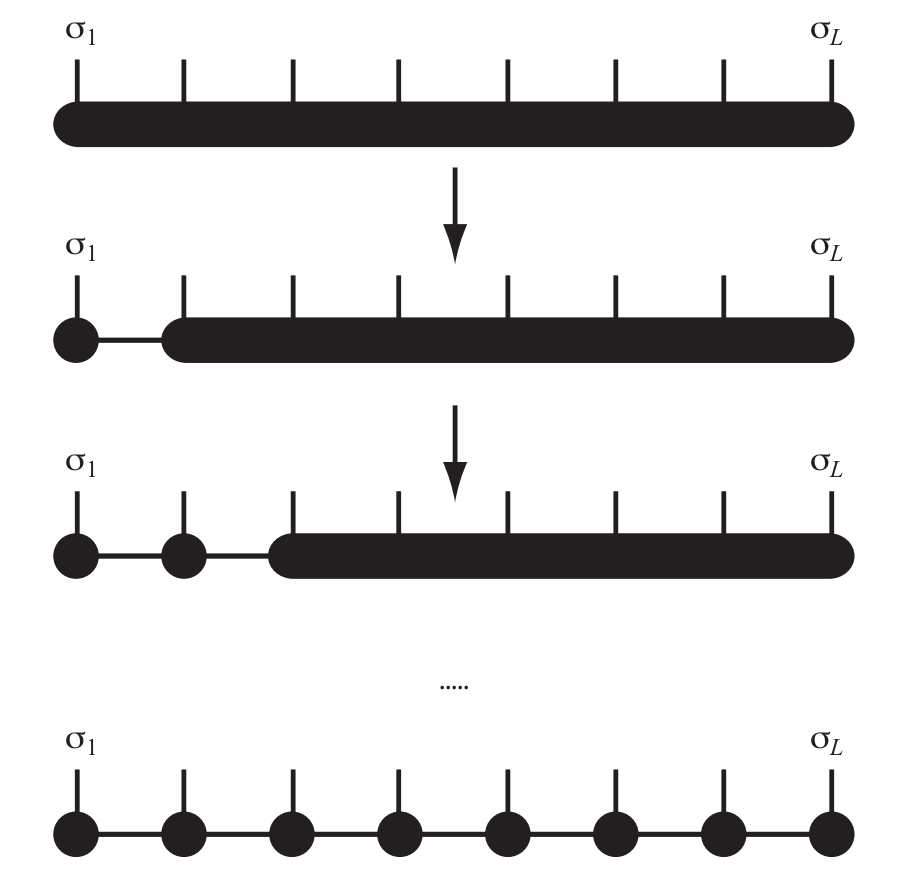
\includegraphics[width=\linewidth]{mps_gen}
\caption{Graphical generation of Matrix Product State from an arbitrary tensor\cite{Schollwock2011}\cite{Orus2014}}
\end{figure}

DMRG constitutes the state of the art for the study of one dimensional quantum lattices.  
The study of the effectiveness of the DMRG algorithm leads naturally to the concept of Matrix Product States(MPS)

The dimension of the product Hilbert space of a spin chain grows exponentially in its length ($\order{d^L}$ where d is the local Hilbert space dimension).
This presents a problem for direct numerical methods. 

However, by an entanglement argument \cite{Orus2014}, we can see that the interesting corner of the total Hilbert space is very small compared to the total space, and in fact this subspace permits an effective numerical description in terms of Matrix Product States.

An arbitrary quantum state can be written
\begin{equation}
    \ket{\psi} = \sum_{\sigma_1, \ldots, \sigma_L} C_{\sigma_1, \ldots, \sigma_L} \ket{\sigma_1, \ldots, \sigma_L},\label{eq:quantum_state}
\end{equation}
Where $\ket{\sigma_i}$ is the local basis of the $ith$ space.
The product states are of the form 
\begin{equation}
    \ket{\psi} = \sum_{\sigma_1, \ldots, \sigma_L} a_{\sigma_1} \ldots c_{\sigma_L} \ket{\sigma_1, \ldots, \sigma_k}
\end{equation}
and have no entanglement structure. 

Via an iterated Singular Value Decomposition (SVD) of the original tensor reshaped into a matrix, we can express eq.\ref{eq:quantum_state} exactly as
\begin{equation}
    \ket{\psi} = \sum_{\sigma_1, \ldots, \sigma_L} A^{\sigma_1} \ldots A^{\sigma_L} \ket{\sigma_1, \ldots, \sigma_L }\label{eq:schollwock_mps}
\end{equation}
or
\begin{equation}
    \ket{\psi} = \sum_{\sigma_1, \ldots, \sigma_L} \Gamma^{\sigma_1}\Lambda_1 \ldots \Lambda_{L-1}\Gamma^{\sigma_L} \ket{\sigma_1, \ldots, \sigma_L }\label{eq:orus_mps}
\end{equation}
Where $A^{\sigma_i}, \Gamma^{\sigma_i}$ denote matrices, and in the second expression $\Lambda_i$ represents the singular values in the ith step of the decomposition.

The index structure of the ($A$ and $\Gamma$) matrices in each of these (exact) expressions goes $(1\times d), (d \times d^2), \ldots (d^2 \times d), (d\times 1)$.

It is a fact from linear algebra that a matrix is optimally approximated in Frobenius norm by its truncated SVD (i.e. $USV^\dagger$ with the smallest singular values set to zero).

Along this line, any state in the total Hilbert space can be systematically approximated by a Matrix Product state of form \ref{eq:orus_mps}, with all but $D$ of the singular values on each site set to zero (for $\Lambda_i$ of dimension $\geq D$)

The 'bond dimension' ($D$) of the MPS can be used to systematically introduce entanglement structure ($D=1$ are the product states).

Your text with scientific results or something... 
Your text with scientific results or something... 
Your text with scientific results or something... 
Your text with scientific results or something... 
Your text with scientific results or something... 
Your text with scientific results or something... 
Your text with scientific results or something... 
Your text with scientific results or something... 
Your text with scientific results or something... 
Your text with scientific results or something... 
Your text with scientific results or something... 
Your text with scientific results or something... 
Your text with scientific results or something... 
Your text with scientific results or something... 
Your text with scientific results or something... 
Your text with scientific results or something... 
Your text with scientific results or something... 
Your text with scientific results or something... 
Your text with scientific results or something... 
Your text with scientific results or something... 

\section{Keldysh Theory}

\begin{figure}[h]
    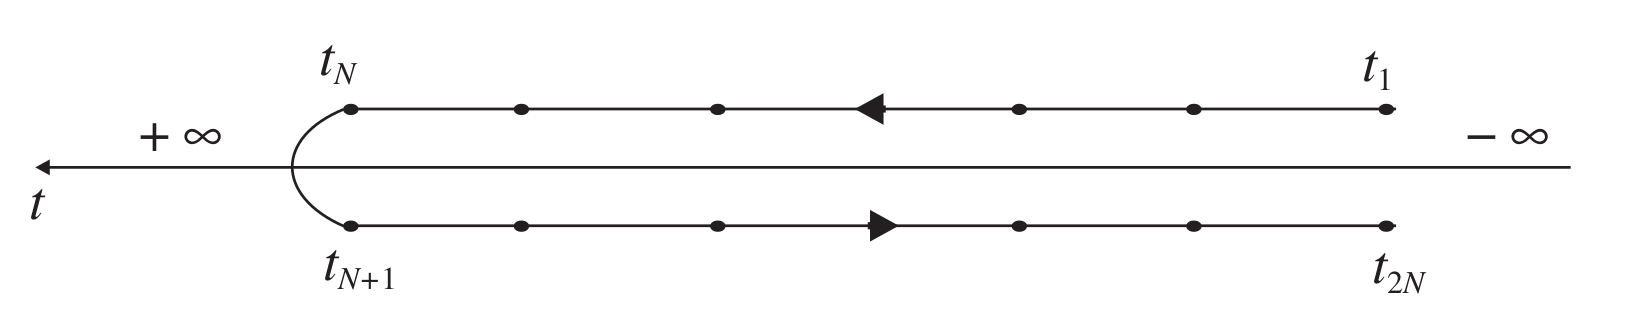
\includegraphics[width=\linewidth]{keldyshcontour}
    \caption{Closed time contour\cite{Kamenev2011}}
\end{figure}
Your text with scientific results or something... 
Your text with scientific results or something... 
Your text with scientific results or something... 
Your text with scientific results or something... 
Your text with scientific results or something... 
Your text with scientific results or something... 
Your text with scientific results or something... 
Your text with scientific results or something... 
Your text with scientific results or something... 
Your text with scientific results or something... 

Your text with scientific results or something... 
Your text with scientific results or something... 
Your text with scientific results or something... 
Your text with scientific results or something... 
Your text with scientific results or something... 
Your text with scientific results or something... 
Your text with scientific results or something... 
Your text with scientific results or something... 
Your text with scientific results or something... 
Your text with scientific results or something... 


%==============================================================================
%==End of content==============================================================
%==============================================================================

%--References------------------------------------------------------------------

\subsection{References}
\bibliography{ref}{}
\bibliographystyle{plain}


\end{multicols}

%==============================================================================
\end{frame}
\end{document}
